\documentclass[12pt]{article}
\usepackage{amsmath}
\usepackage{tikz}
\usepackage{pgfplots}

\pgfplotsset{compat=1.17}

\begin{document}

\title{Understanding\\the Standard Form\\of Linear Equations}
\author{Tutoring Centre Ferndale}
\date{}
\maketitle

In linear algebra, the slope-intercept form \(y = mx + b\) is often preferred for its intuitive representation of the slope (\(m\)) and the y-intercept (\(b\)). However, the standard form of a linear equation, \(Ax + By = C\), provides a different perspective on linear relationships. Understanding how changes in \(A\), \(B\), and \(C\) affect the graph can offer valuable insights.

\section*{Standard Form: \(Ax + By = C\)}

In the standard form, \(Ax + By = C\):
\begin{itemize}
    \item \(A\), \(B\), and \(C\) are constants.
    \item \(A\) and \(B\) determine the slope and orientation of the line.
    \item \(C\) affects the position of the line without changing its slope.
\end{itemize}

\subsection*{Questions}
\begin{enumerate}
    \item What are the constants in the standard form \(Ax + By = C\)?
    \item How do \(A\) and \(B\) influence the line in standard form?
    \item What is the role of \(C\) in the standard form?
\end{enumerate}

\newpage

\section*{Effect of Changing \(C\)}

\begin{itemize}
    \item \(C\) affects the line's position but not its slope.
    \item Increasing \(C\) shifts the line upwards or to the right, while decreasing \(C\) shifts it downwards or to the left.
    \item The line remains parallel to its original position because the slope, given by \(-A/B\), remains unchanged.
\end{itemize}

\subsection*{Example}

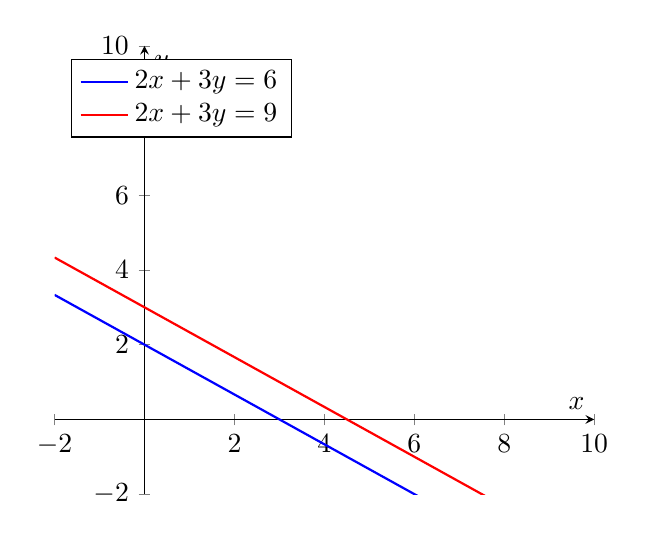
\begin{tikzpicture}
    \begin{axis}[
        axis lines = middle,
        xlabel = {$x$},
        ylabel = {$y$},
        ymin=-2, ymax=10,
        xmin=-2, xmax=10,
        domain=-2:10,
        samples=100,
        legend pos=north west
    ]
    \addplot [blue, thick] {(-2*x + 6)/3};
    \addplot [red, thick] {(-2*x + 9)/3};
    \legend{$2x + 3y = 6$, $2x + 3y = 9$}
    \end{axis}
\end{tikzpicture}

+The new line \(2x + 3y = 9\) is parallel to \(2x + 3y = 6\) but shifted upwards or to the right.

\subsection*{Questions}
\begin{enumerate}
    \item How does increasing \(C\) affect the line's position?
    \item How does decreasing \(C\) affect the line's position?
    \item Does the slope of the line change when \(C\) changes?
\end{enumerate}

\newpage

\section*{Effect of Changing \(A\)}

\begin{itemize}
    \item \(A\) influences the slope and x-intercept.
    \item Increasing \(A\) makes the line steeper in the x-direction, while decreasing \(A\) makes it less steep.
\end{itemize}

\subsection*{Example}

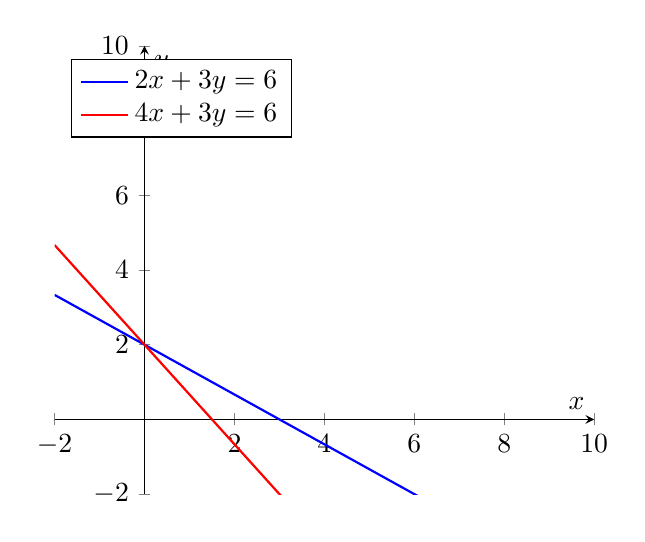
\begin{tikzpicture}
    \begin{axis}[
        axis lines = middle,
        xlabel = {$x$},
        ylabel = {$y$},
        ymin=-2, ymax=10,
        xmin=-2, xmax=10,
        domain=-2:10,
        samples=100,
        legend pos=north west
    ]
    \addplot [blue, thick] {(-2*x + 6)/3};
    \addplot [red, thick] {(-4*x + 6)/3};
    \legend{$2x + 3y = 6$, $4x + 3y = 6$}
    \end{axis}
\end{tikzpicture}

The new line \(4x + 3y = 6\) is steeper in the x-direction compared to \(2x + 3y = 6\).

\subsection*{Questions}
\begin{enumerate}
    \item How does increasing \(A\) affect the line's steepness?
    \item How does decreasing \(A\) affect the line's steepness?
    \item What happens to the x-intercept when \(A\) changes?
\end{enumerate}

\newpage

\section*{Effect of Changing \(B\)}

\begin{itemize}
    \item \(B\) influences the slope and y-intercept.
    \item Increasing \(B\) makes the line less steep in the y-direction, while decreasing \(B\) makes it steeper.
\end{itemize}

\subsection*{Example}

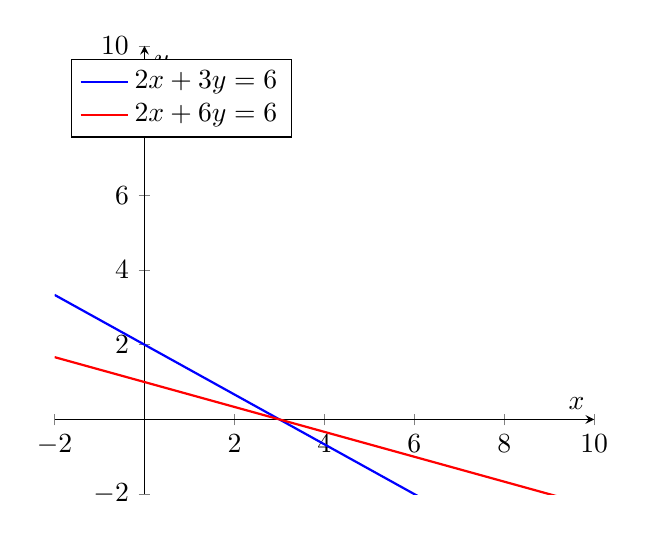
\begin{tikzpicture}
    \begin{axis}[
        axis lines = middle,
        xlabel = {$x$},
        ylabel = {$y$},
        ymin=-2, ymax=10,
        xmin=-2, xmax=10,
        domain=-2:10,
        samples=100,
        legend pos=north west
    ]
    \addplot [blue, thick] {(-2*x + 6)/3};
    \addplot [red, thick] {(-2*x + 6)/6};
    \legend{$2x + 3y = 6$, $2x + 6y = 6$}
    \end{axis}
\end{tikzpicture}

The new line \(2x + 6y = 6\) is less steep in the y-direction compared to \(2x + 3y = 6\).

\subsection*{Questions}
\begin{enumerate}
    \item How does increasing \(B\) affect the line's steepness?
    \item How does decreasing \(B\) affect the line's steepness?
    \item What happens to the y-intercept when \(B\) changes?
\end{enumerate}

\newpage

\section*{Converting Between Forms}

To fully appreciate the effects, it can be helpful to convert the standard form \(Ax + By = C\) to the slope-intercept form \(y = mx + b\):

\[
Ax + By = C
\]
\[
By = -Ax + C
\]
\[
y = -\frac{A}{B}x + \frac{C}{B}
\]

Here, the slope \(m\) is \(-\frac{A}{B}\), and the y-intercept \(b\) is \(\frac{C}{B}\).

\subsection*{Questions}
\begin{enumerate}
    \item What is the slope in the slope-intercept form derived from \(Ax + By = C\)?
    \item What is the y-intercept in the slope-intercept form derived from \(Ax + By = C\)?
    \item Convert the standard form \(4x + 5y = 20\) to the slope-intercept form.

\section*{Summary}

\begin{itemize}
    \item \textbf{Changing \(C\)} shifts the line without altering its slope.
    \item \textbf{Changing \(A\)} adjusts the line's steepness in the x-direction.
    \item \textbf{Changing \(B\)} adjusts the line's steepness in the y-direction.
\end{itemize}

Understanding these effects can help in analyzing and graphing linear equations in standard form. Each parameter plays a unique role in defining the line's properties and behavior on the Cartesian plane.

\newpage

\section*{Answers}

\subsection*{Standard Form: \(Ax + By = C\)}
\begin{enumerate}
    \item The constants are \(A\), \(B\), and \(C\).
    \item \(A\) and \(B\) influence the slope and orientation of the line.
    \item \(C\) affects the position of the line without changing its slope.
\end{enumerate}

\subsection*{Effect of Changing \(C\)}
\begin{enumerate}
    \item Increasing \(C\) shifts the line upwards or to the right.
    \item Decreasing \(C\) shifts the line downwards or to the left.
    \item The slope of the line does not change when \(C\) changes.
\end{enumerate}

\subsection*{Effect of Changing \(A\)}
\begin{enumerate}
    \item Increasing \(A\) makes the line steeper in the x-direction.
    \item Decreasing \(A\) makes the line less steep in the x-direction.
    \item The x-intercept changes as \(A\) changes.
\end{enumerate}

\subsection*{Effect of Changing \(B\)}
\begin{enumerate}
    \item Increasing \(B\) makes the line less steep in the y-direction.
    \item Decreasing \(B\) makes the line steeper in the y-direction.
    \item The y-intercept changes as \(B\) changes.
\end{enumerate}

\subsection*{Converting Between Forms}
\begin{enumerate}
    \item The slope is \(-\frac{A}{B}\).
    \item The y-intercept is \(\frac{C}{B}\).
    \item Converting \(4x + 5y = 20\) to slope-intercept form:
   \[
   5y = -4x + 20
   \]
   \[
   y = -\frac{4}{5}x + 4
   \]
\end{enumerate}

\end{document}
